\subsection{Эффект Доплера. Красное смещение} 
\textit{Эффект Доплера} --- изменение частоты и длины волны, регистрируемых  приёмником, вызванное движением их источника и/или движением приёмника (Рис.\ref{doppler-ef}).

\begin{figure}[h!]\centering
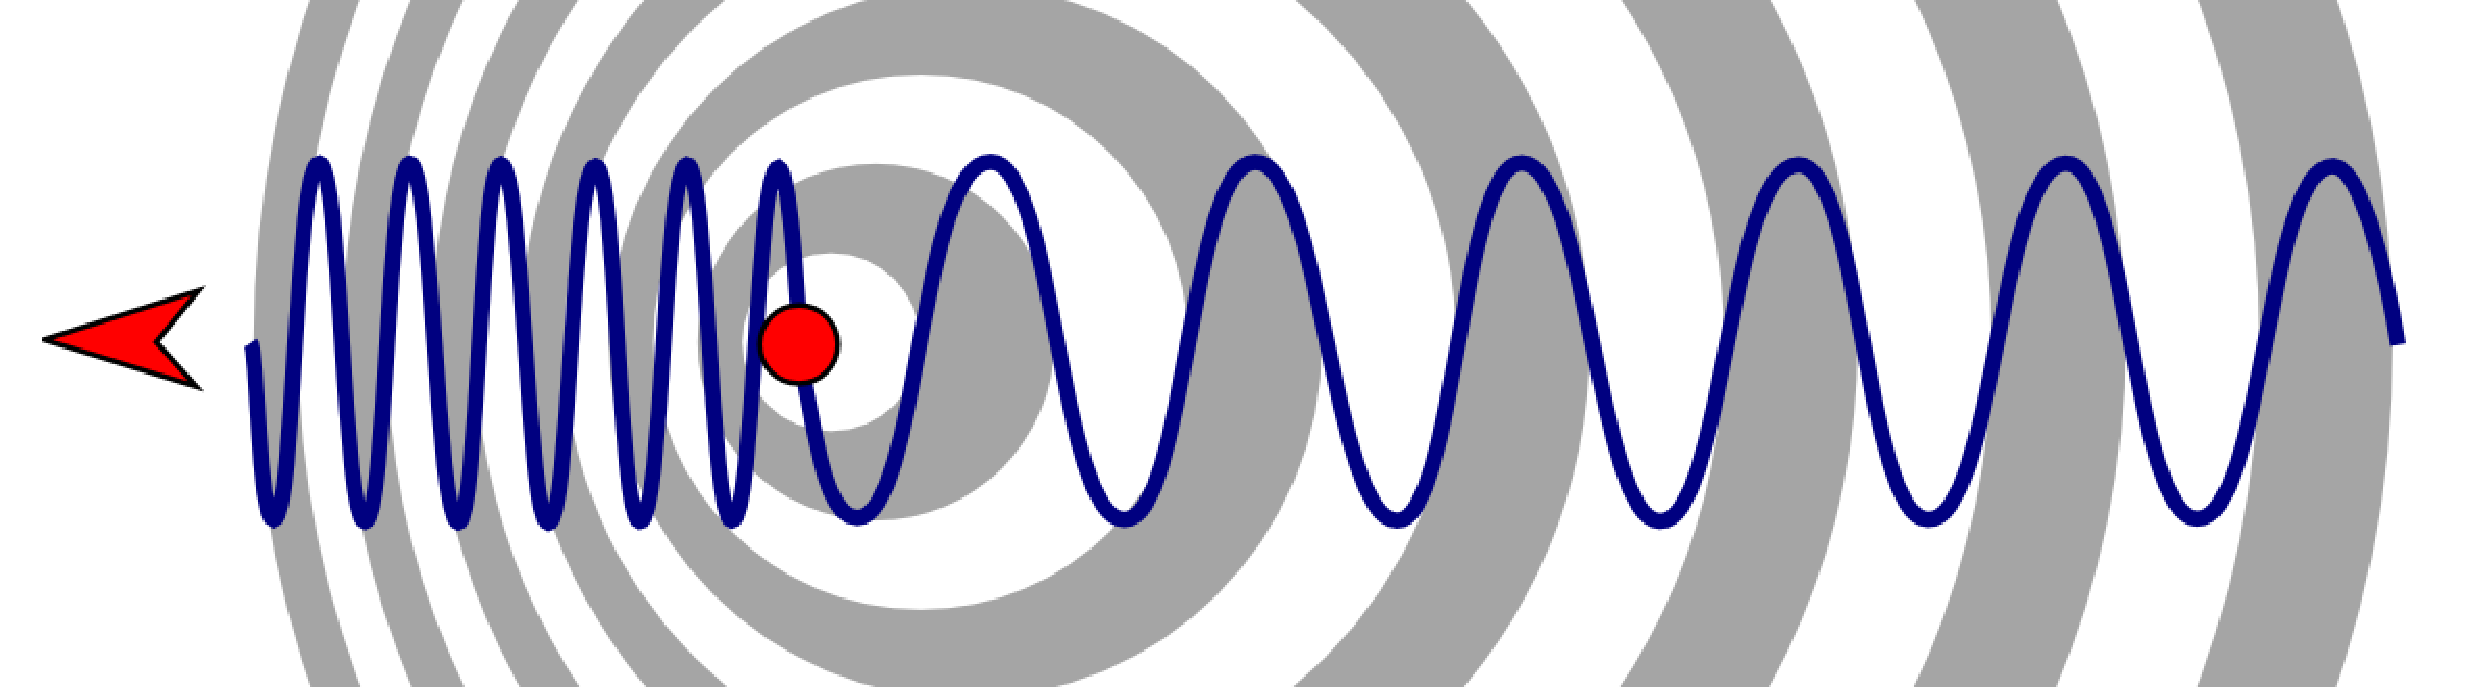
\includegraphics[width=0.5\textwidth]{doppler-ef}
\caption{Эффект Доплера}\label{doppler-ef}
\end{figure}

Формулу для релятивистского эффекта Доплера выводят из уравнений  специальной теории относительности и обусловлена она двумя причинами:
\begin{enumerate}
\item Классический аналог изменения частоты при относительном движении источника и приёмника.
\item Релятивистское замедление времени.
\end{enumerate}

Записывается он следующим образом:
\begin{equation}
\nu=\nu_0\cdot\frac{\sqrt{1-\frac{v^2}{c^2}}}{1-\frac{v}{c}\cdot\cos\theta},
\end{equation}
где $\nu$--- частота, с которой наблюдатель принимает волны, $\nu_0$ --- частота, с которой источник испускает волны, $v$ --- скорость источника, $\theta$ --- угол между направлением на источник и вектором скорости в системе отсчёта приёмника. 

Если источник радиально удаляется от наблюдателя, то $\theta =0$, если приближается, то $\theta =\pi$.

\textit{Красное смещение} --- сдвиг спектральных линий химических элементов в красную (длинноволновую) сторону. Оно показывает скорость удаления и расстояние до галактик или других объектов. Параметр красного смещения определяется таким образом:
\begin{equation}
z=\frac{\lambda-\lambda_0}{\lambda_0},
\end{equation}
где $\lambda$ и $\lambda _{0}$ --- значения длины волны в точках наблюдения и испускания излучения соответственно.

Доплеровское смещение длины волны в спектре источника, движущегося с лучевой скоростью $v_{r}$ и полной скоростью $v$, равно:
\begin{equation}
z_D=\frac{1+\frac{v_r}{c}}{\sqrt{1-\left(\frac{v}{c}\right)^2}}
\end{equation}

\textit{Гравитационное красное смещение} --- проявление эффекта изменения частоты испущенного некоторым источником света по мере удаления от массивных объектов, таких как звёзды и чёрные дыры; оно наблюдается как сдвиг спектральных линий в излучении источников, близких к массивным телам, в красную область спектра. Через длины волн и частоты записывается как:
\begin{equation}
Z_D=\frac{\lambda-\lambda_0}{\lambda_0}=\frac{\nu-\nu_0}{\nu_0}
\end{equation}

Также гравитационное красное смещение определяется из формулы, выведенной Эйнштейном:
\begin{equation}
Z_G=\frac{GM}{c^2r}-\frac{GM}{c^2R}\approx\frac{GM}{c^2r}, 
\end{equation}
т.к. $GM/c^2r\ll GM/c^2R$, где $M$ --- масса гравитирующего тела, $r$ --- радиальное расстояние от центра масс тела до точки излучения, $R$ ---  радиальное расстояние от центра масс тела до точки наблюдения.
